\chapter{Lisää segmenttipuusta}

Segmenttipuu on tehokas tietorakenne,
joka mahdollistaa monenlaisten
kyselyiden toteuttamisen tehokkaasti.
Tähän mennessä olemme käyttäneet
kuitenkin segmenttipuuta melko rajoittuneesti.
Nyt on aika tutustua pintaa syvemmältä
segmenttipuun mahdollisuuksiin.

Tähän mennessä olemme kulkeneet segmenttipuuta
\textit{alhaalta ylöspäin} lehdistä juureen.
Vaihtoehtoinen tapa toteuttaa puun käsittely
on kulkea \textit{ylhäältä alaspäin} juuresta lehtiin.
Tämä kulkusuunta on usein kätevä silloin,
kun kyseessä on perustilannetta
monimutkaisempi segmenttipuu.

Esimerkiksi välin $[a,b]$ summan laskeminen
segmenttipuussa tapahtuu alhaalta ylöspäin 
tuttuun tapaan näin (luku 9.3):

\begin{lstlisting}
int summa(int a, int b) {
    a += N; b += N;
    int s = 0;
    while (a <= b) {
        if (a%2 == 1) s += p[a++];
        if (b%2 == 0) s += p[b--];
        a /= 2; b /= 2;
    }
    return s;
}
\end{lstlisting}
Ylhäältä alaspäin toteutettuna funktiosta tulee:

\begin{lstlisting}
int summa(int a, int b, int k, int c, int d) {
    if (b < c || a > d) return 0;
    if (a == c && b == d) return p[k];
    int w = (d-c+1)/2;
    return summa(a, min(c+w-1,b), 2*k, a, a+w-1) +
           summa(max(c+w,a), b, 2*k+1, a+w, b);
}
\end{lstlisting}
Nyt välin $[a,b]$ summan saa laskettua
kutsumalla funktiota näin:

\begin{lstlisting}
int s = summa(a, b, 1, 0, N-1);
\end{lstlisting}

Parametri $k$ ilmaisee kohdan
taulukossa \texttt{p}.
Aluksi $k$:n arvona on 1,
koska summan laskeminen alkaa
segmenttipuun juuresta.

Väli $[c,d]$ on parametria $k$ vastaava väli,
aluksi koko kyselyalue eli $[0,N-1]$.
Jos väli $[a,b]$ on välin $[c,d]$
ulkopuolella, välin summa on 0.
Jos taas välit $[a,b]$ ja $[c,d]$
ovat samat, summan saa taulukosta \texttt{p}.

Jos väli $[a,b]$ on kokonaan tai osittain välin $[c,d]$
sisällä, haku jatkuu rekursiivisesti
välin $[c,d]$ vasemmasta ja oikeasta puoliskosta.
Kummankin puoliskon koko on $w=(d-c+1)/2$,
joten vasen puolisko kattaa välin $[c,c+w/2-1]$
ja oikea puolisko kattaa välin $[c+w/2,d]$.

Seuraava kuva näyttää,
kuinka haku etenee puussa,
kun lasketaan puun alle
merkityn välin summa.
Harmaat solmut ovat kohtia,
joissa rekursio päättyy ja välin
summan saa taulukosta \texttt{p}.
\\
\begin{center}
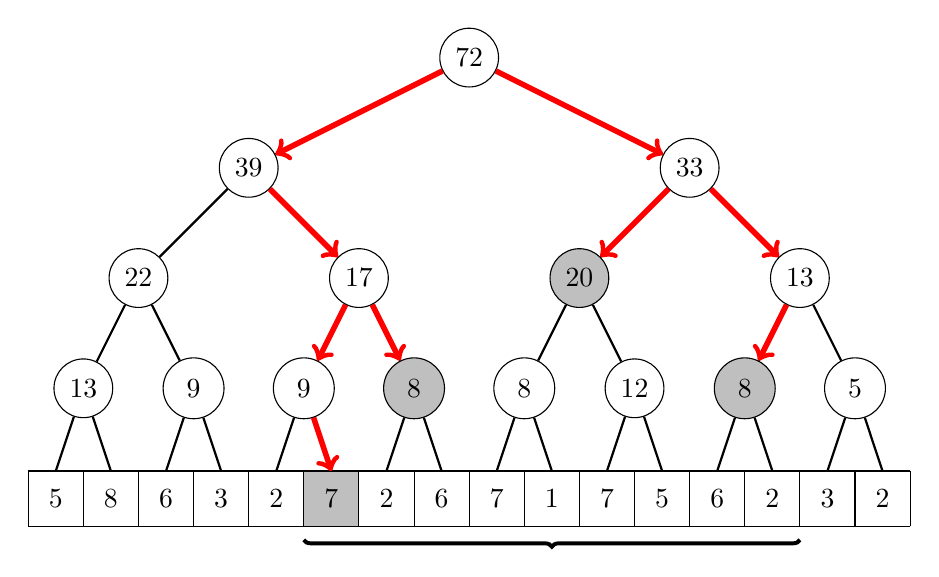
\begin{tikzpicture}[scale=0.7]
\fill[color=gray!50] (5,0) rectangle (6,1);
\draw (0,0) grid (16,1);

\node[anchor=center] at (0.5, 0.5) {5};
\node[anchor=center] at (1.5, 0.5) {8};
\node[anchor=center] at (2.5, 0.5) {6};
\node[anchor=center] at (3.5, 0.5) {3};
\node[anchor=center] at (4.5, 0.5) {2};
\node[anchor=center] at (5.5, 0.5) {7};
\node[anchor=center] at (6.5, 0.5) {2};
\node[anchor=center] at (7.5, 0.5) {6};
\node[anchor=center] at (8.5, 0.5) {7};
\node[anchor=center] at (9.5, 0.5) {1};
\node[anchor=center] at (10.5, 0.5) {7};
\node[anchor=center] at (11.5, 0.5) {5};
\node[anchor=center] at (12.5, 0.5) {6};
\node[anchor=center] at (13.5, 0.5) {2};
\node[anchor=center] at (14.5, 0.5) {3};
\node[anchor=center] at (15.5, 0.5) {2};

%\node[anchor=center] at (1,2.5) {13};

\node[draw, circle] (a) at (1,2.5) {13};
\path[draw,thick,-] (a) -- (0.5,1);
\path[draw,thick,-] (a) -- (1.5,1);
\node[draw, circle,minimum size=22pt] (b) at (3,2.5) {9};
\path[draw,thick,-] (b) -- (2.5,1);
\path[draw,thick,-] (b) -- (3.5,1);
\node[draw, circle,minimum size=22pt] (c) at (5,2.5) {9};
\path[draw,thick,-] (c) -- (4.5,1);
\path[draw,thick,-] (c) -- (5.5,1);
\node[draw, circle,fill=gray!50,minimum size=22pt] (d) at (7,2.5) {8};
\path[draw,thick,-] (d) -- (6.5,1);
\path[draw,thick,-] (d) -- (7.5,1);
\node[draw, circle,minimum size=22pt] (e) at (9,2.5) {8};
\path[draw,thick,-] (e) -- (8.5,1);
\path[draw,thick,-] (e) -- (9.5,1);
\node[draw, circle] (f) at (11,2.5) {12};
\path[draw,thick,-] (f) -- (10.5,1);
\path[draw,thick,-] (f) -- (11.5,1);
\node[draw, circle,fill=gray!50,minimum size=22pt] (g) at (13,2.5) {8};
\path[draw,thick,-] (g) -- (12.5,1);
\path[draw,thick,-] (g) -- (13.5,1);
\node[draw, circle,minimum size=22pt] (h) at (15,2.5) {5};
\path[draw,thick,-] (h) -- (14.5,1);
\path[draw,thick,-] (h) -- (15.5,1);

\node[draw, circle] (i) at (2,4.5) {22};
\path[draw,thick,-] (i) -- (a);
\path[draw,thick,-] (i) -- (b);
\node[draw, circle] (j) at (6,4.5) {17};
\path[draw,thick,-] (j) -- (c);
\path[draw,thick,-] (j) -- (d);
\node[draw, circle,fill=gray!50] (k) at (10,4.5) {20};
\path[draw,thick,-] (k) -- (e);
\path[draw,thick,-] (k) -- (f);
\node[draw, circle] (l) at (14,4.5) {13};
\path[draw,thick,-] (l) -- (g);
\path[draw,thick,-] (l) -- (h);

\node[draw, circle] (m) at (4,6.5) {39};
\path[draw,thick,-] (m) -- (i);
\path[draw,thick,-] (m) -- (j);
\node[draw, circle] (n) at (12,6.5) {33};
\path[draw,thick,-] (n) -- (k);
\path[draw,thick,-] (n) -- (l);

\node[draw, circle] (o) at (8,8.5) {72};
\path[draw,thick,-] (o) -- (m);
\path[draw,thick,-] (o) -- (n);

\path[draw=red,thick,->,line width=2pt] (o) -- (m);
\path[draw=red,thick,->,line width=2pt] (o) -- (n);

\path[draw=red,thick,->,line width=2pt] (m) -- (j);
\path[draw=red,thick,->,line width=2pt] (j) -- (c);
\path[draw=red,thick,->,line width=2pt] (j) -- (d);
\path[draw=red,thick,->,line width=2pt] (c) -- (5.5,1);

\path[draw=red,thick,->,line width=2pt] (n) -- (k);
\path[draw=red,thick,->,line width=2pt] (n) -- (l);

\path[draw=red,thick,->,line width=2pt] (l) -- (g);

\draw [decoration={brace}, decorate, line width=0.5mm] (14,-0.25) -- (5,-0.25);
\end{tikzpicture}
\end{center}
Myös tässä toteutuksessa kyselyn aikavaativuus on $O(\log n)$,
koska haun aikana käsiteltävien solmujen määrä on $O(\log n)$.

\section{Laiska eteneminen}

Laiska eteneminen (\textit{lazy propagation})
mahdollistaa segmenttipuun,
jossa voi sekä muuttaa väliä että kysyä tietoa väliltä
ajassa $O(\log n)$.
Ideana on suorittaa muutokset ja kyselyt ylhäältä
alaspäin ja toteuttaa muutokset laiskasti niin,
että ne välitetään puussa alaspäin vain silloin,
kun se on välttämätöntä.

Laiskassa segmenttipuussa solmuihin liittyy
kahdenlaista tietoa.
Kuten tavallisessa segmenttipuussa,
jokaisessa solmussa on sitä vastaavan välin
summa tai muu haluttu tieto.
Tämän lisäksi solmussa voi olla laiskaan etenemiseen
liittyvää tietoa, jota ei ole vielä välitetty
solmusta alaspäin.

Välin muutostapa voi olla joko
\textit{lisäys} tai \textit{asetus}.
Lisäyksessä välin jokaiseen alkioon lisätään
tietty arvo, ja asetuksessa välin
jokainen alkio saa tietyn arvon.
Kummankin operaation toteutus on melko samanlainen,
ja puu voi myös sallia samaan aikaan
molemmat muutostavat.

\subsubsection{Laiska segmenttipuu}

Tarkastellaan esimerkkinä tilannetta,
jossa segmenttipuun
tulee toteuttaa seuraavat operaatiot:
\begin{itemize}
\item lisää jokaisen välin $[a,b]$ alkioon arvo $x$
\item laske välin $[a,b]$ alkioiden summa
\end{itemize}
Toteutamme puun, jonka jokaisessa
solmussa on kaksi arvoa $s/z$:
välin lukujen summa $s$,
kuten tavallisessa segmenttipuussa, sekä
laiska muutos $z$,
joka tarkoittaa,
että kaikkiin välin lukuihin tulee lisätä $z$.
Seuraavassa puussa jokaisessa solmussa $z=0$
eli mitään muutoksia ei ole kesken.
\begin{center}
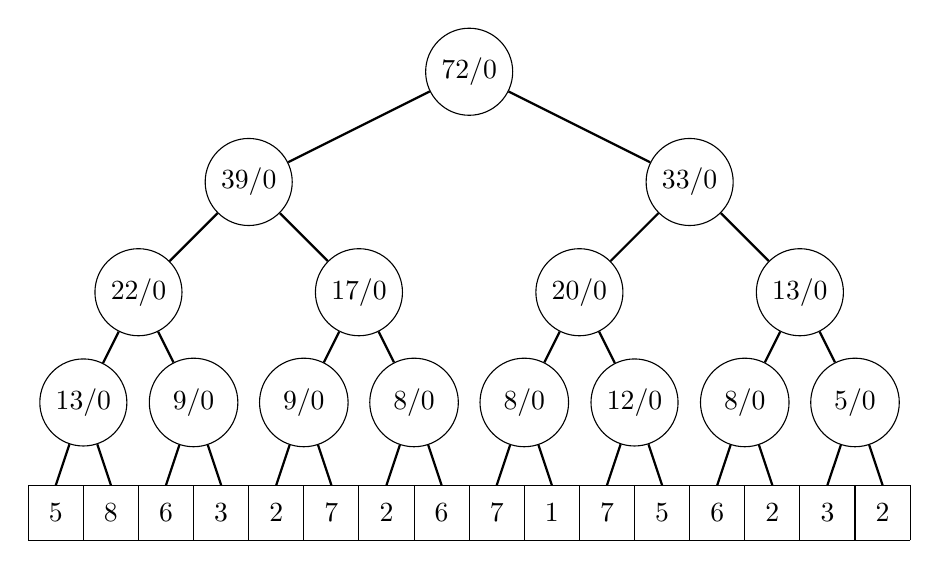
\begin{tikzpicture}[scale=0.7]
\draw (0,0) grid (16,1);

\node[anchor=center] at (0.5, 0.5) {5};
\node[anchor=center] at (1.5, 0.5) {8};
\node[anchor=center] at (2.5, 0.5) {6};
\node[anchor=center] at (3.5, 0.5) {3};
\node[anchor=center] at (4.5, 0.5) {2};
\node[anchor=center] at (5.5, 0.5) {7};
\node[anchor=center] at (6.5, 0.5) {2};
\node[anchor=center] at (7.5, 0.5) {6};
\node[anchor=center] at (8.5, 0.5) {7};
\node[anchor=center] at (9.5, 0.5) {1};
\node[anchor=center] at (10.5, 0.5) {7};
\node[anchor=center] at (11.5, 0.5) {5};
\node[anchor=center] at (12.5, 0.5) {6};
\node[anchor=center] at (13.5, 0.5) {2};
\node[anchor=center] at (14.5, 0.5) {3};
\node[anchor=center] at (15.5, 0.5) {2};

\node[draw, circle] (a) at (1,2.5) {13/0};
\path[draw,thick,-] (a) -- (0.5,1);
\path[draw,thick,-] (a) -- (1.5,1);
\node[draw, circle,minimum size=32pt] (b) at (3,2.5) {9/0};
\path[draw,thick,-] (b) -- (2.5,1);
\path[draw,thick,-] (b) -- (3.5,1);
\node[draw, circle,minimum size=32pt] (c) at (5,2.5) {9/0};
\path[draw,thick,-] (c) -- (4.5,1);
\path[draw,thick,-] (c) -- (5.5,1);
\node[draw, circle,minimum size=32pt] (d) at (7,2.5) {8/0};
\path[draw,thick,-] (d) -- (6.5,1);
\path[draw,thick,-] (d) -- (7.5,1);
\node[draw, circle,minimum size=32pt] (e) at (9,2.5) {8/0};
\path[draw,thick,-] (e) -- (8.5,1);
\path[draw,thick,-] (e) -- (9.5,1);
\node[draw, circle] (f) at (11,2.5) {12/0};
\path[draw,thick,-] (f) -- (10.5,1);
\path[draw,thick,-] (f) -- (11.5,1);
\node[draw, circle,minimum size=32pt] (g) at (13,2.5) {8/0};
\path[draw,thick,-] (g) -- (12.5,1);
\path[draw,thick,-] (g) -- (13.5,1);
\node[draw, circle,minimum size=32pt] (h) at (15,2.5) {5/0};
\path[draw,thick,-] (h) -- (14.5,1);
\path[draw,thick,-] (h) -- (15.5,1);

\node[draw, circle] (i) at (2,4.5) {22/0};
\path[draw,thick,-] (i) -- (a);
\path[draw,thick,-] (i) -- (b);
\node[draw, circle] (j) at (6,4.5) {17/0};
\path[draw,thick,-] (j) -- (c);
\path[draw,thick,-] (j) -- (d);
\node[draw, circle] (k) at (10,4.5) {20/0};
\path[draw,thick,-] (k) -- (e);
\path[draw,thick,-] (k) -- (f);
\node[draw, circle] (l) at (14,4.5) {13/0};
\path[draw,thick,-] (l) -- (g);
\path[draw,thick,-] (l) -- (h);

\node[draw, circle] (m) at (4,6.5) {39/0};
\path[draw,thick,-] (m) -- (i);
\path[draw,thick,-] (m) -- (j);
\node[draw, circle] (n) at (12,6.5) {33/0};
\path[draw,thick,-] (n) -- (k);
\path[draw,thick,-] (n) -- (l);

\node[draw, circle] (o) at (8,8.5) {72/0};
\path[draw,thick,-] (o) -- (m);
\path[draw,thick,-] (o) -- (n);
\end{tikzpicture}
\end{center}

Kun välin $[a,b]$ solmuja kasvatetaan $x$:llä,
alkaa kulku puun juuresta lehtiä kohti.
Kulun aikana tapahtuu kahdenlaisia muutoksia puun solmuihin:

Jos solmun väli $[c,d]$ kuuluu kokonaan
muutettavalle välille $[a,b]$,
solmun $z$-arvo kasvaa $x$:llä ja kulku pysähtyy.
Jos taas väli $[c,d]$ kuuluu osittain välille $[a,b]$,
solmun $s$-arvo kasvaa $hx$:llä,
missä $h$ on välien $[a,b]$ ja $[c,d]$ yhteisen osan pituus,
ja kulku jatkuu rekursiivisesti alaspäin.

Kasvatetaan esimerkiksi puun alle merkittyä väliä 2:lla:
\begin{center}
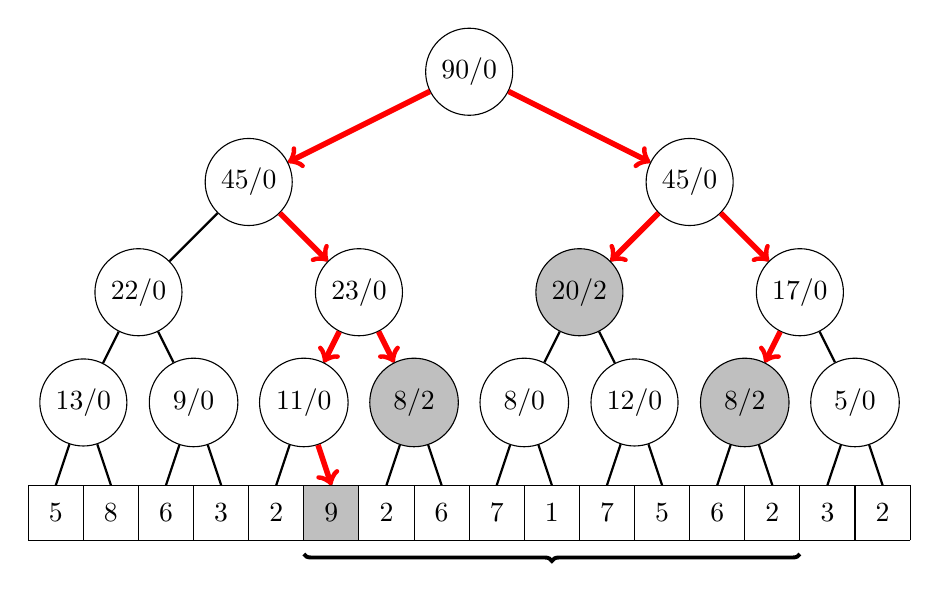
\begin{tikzpicture}[scale=0.7]
\fill[color=gray!50] (5,0) rectangle (6,1);
\draw (0,0) grid (16,1);

\node[anchor=center] at (0.5, 0.5) {5};
\node[anchor=center] at (1.5, 0.5) {8};
\node[anchor=center] at (2.5, 0.5) {6};
\node[anchor=center] at (3.5, 0.5) {3};
\node[anchor=center] at (4.5, 0.5) {2};
\node[anchor=center] at (5.5, 0.5) {9};
\node[anchor=center] at (6.5, 0.5) {2};
\node[anchor=center] at (7.5, 0.5) {6};
\node[anchor=center] at (8.5, 0.5) {7};
\node[anchor=center] at (9.5, 0.5) {1};
\node[anchor=center] at (10.5, 0.5) {7};
\node[anchor=center] at (11.5, 0.5) {5};
\node[anchor=center] at (12.5, 0.5) {6};
\node[anchor=center] at (13.5, 0.5) {2};
\node[anchor=center] at (14.5, 0.5) {3};
\node[anchor=center] at (15.5, 0.5) {2};

\node[draw, circle] (a) at (1,2.5) {13/0};
\path[draw,thick,-] (a) -- (0.5,1);
\path[draw,thick,-] (a) -- (1.5,1);
\node[draw, circle,minimum size=32pt] (b) at (3,2.5) {9/0};
\path[draw,thick,-] (b) -- (2.5,1);
\path[draw,thick,-] (b) -- (3.5,1);
\node[draw, circle,minimum size=32pt] (c) at (5,2.5) {11/0};
\path[draw,thick,-] (c) -- (4.5,1);
\path[draw,thick,-] (c) -- (5.5,1);
\node[draw, circle,fill=gray!50,minimum size=32pt] (d) at (7,2.5) {8/2};
\path[draw,thick,-] (d) -- (6.5,1);
\path[draw,thick,-] (d) -- (7.5,1);
\node[draw, circle,minimum size=32pt] (e) at (9,2.5) {8/0};
\path[draw,thick,-] (e) -- (8.5,1);
\path[draw,thick,-] (e) -- (9.5,1);
\node[draw, circle] (f) at (11,2.5) {12/0};
\path[draw,thick,-] (f) -- (10.5,1);
\path[draw,thick,-] (f) -- (11.5,1);
\node[draw, circle,fill=gray!50,minimum size=32pt] (g) at (13,2.5) {8/2};
\path[draw,thick,-] (g) -- (12.5,1);
\path[draw,thick,-] (g) -- (13.5,1);
\node[draw, circle,minimum size=32pt] (h) at (15,2.5) {5/0};
\path[draw,thick,-] (h) -- (14.5,1);
\path[draw,thick,-] (h) -- (15.5,1);

\node[draw, circle] (i) at (2,4.5) {22/0};
\path[draw,thick,-] (i) -- (a);
\path[draw,thick,-] (i) -- (b);
\node[draw, circle] (j) at (6,4.5) {23/0};
\path[draw,thick,-] (j) -- (c);
\path[draw,thick,-] (j) -- (d);
\node[draw, circle,fill=gray!50] (k) at (10,4.5) {20/2};
\path[draw,thick,-] (k) -- (e);
\path[draw,thick,-] (k) -- (f);
\node[draw, circle] (l) at (14,4.5) {17/0};
\path[draw,thick,-] (l) -- (g);
\path[draw,thick,-] (l) -- (h);

\node[draw, circle] (m) at (4,6.5) {45/0};
\path[draw,thick,-] (m) -- (i);
\path[draw,thick,-] (m) -- (j);
\node[draw, circle] (n) at (12,6.5) {45/0};
\path[draw,thick,-] (n) -- (k);
\path[draw,thick,-] (n) -- (l);

\node[draw, circle] (o) at (8,8.5) {90/0};
\path[draw,thick,-] (o) -- (m);
\path[draw,thick,-] (o) -- (n);

\path[draw=red,thick,->,line width=2pt] (o) -- (m);
\path[draw=red,thick,->,line width=2pt] (o) -- (n);

\path[draw=red,thick,->,line width=2pt] (m) -- (j);
\path[draw=red,thick,->,line width=2pt] (j) -- (c);
\path[draw=red,thick,->,line width=2pt] (j) -- (d);
\path[draw=red,thick,->,line width=2pt] (c) -- (5.5,1);

\path[draw=red,thick,->,line width=2pt] (n) -- (k);
\path[draw=red,thick,->,line width=2pt] (n) -- (l);

\path[draw=red,thick,->,line width=2pt] (l) -- (g);

\draw [decoration={brace}, decorate, line width=0.5mm] (14,-0.25) -- (5,-0.25);
\end{tikzpicture}
\end{center}

Välin $[a,b]$ summan laskenta tapahtuu myös
kulkuna puun juuresta lehtiä kohti.
Jos solmun väli $[c,d]$ kuuluu kokonaan väliin $[a,b]$,
kyselyn summaan lisätään solmun $s$-arvo
sekä mahdollinen $z$-arvon tuottama lisäys.
Muussa tapauksessa kulku jatkuu rekursiivisesti alaspäin solmun lapsiin.

Aina ennen solmun käsittelyä siinä mahdollisesti
oleva laiska muutos välitetään tasoa alemmas.
Tämä tapahtuu sekä välin muutoskyselyssä
että summakyselyssä.
Ideana on, että laiska muutos etenee alaspäin
vain silloin, kun tämä on välttämätöntä,
jotta puun käsittely on tehokasta.

Seuraava kuva näyttää, kuinka äskeinen puu muuttuu,
kun siitä lasketaan puun alapuolelle merkityn välin summa:
\begin{center}
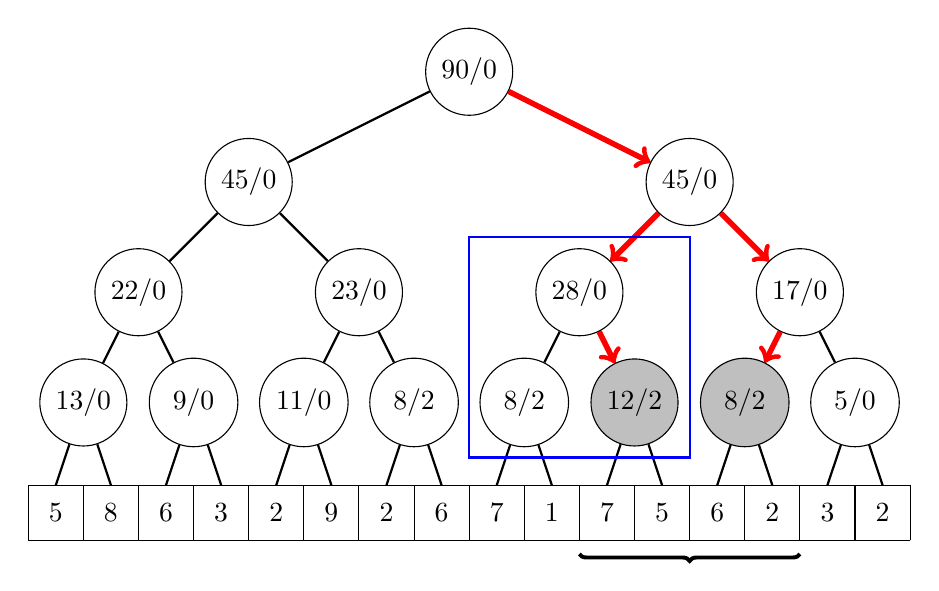
\begin{tikzpicture}[scale=0.7]
\draw (0,0) grid (16,1);

\node[anchor=center] at (0.5, 0.5) {5};
\node[anchor=center] at (1.5, 0.5) {8};
\node[anchor=center] at (2.5, 0.5) {6};
\node[anchor=center] at (3.5, 0.5) {3};
\node[anchor=center] at (4.5, 0.5) {2};
\node[anchor=center] at (5.5, 0.5) {9};
\node[anchor=center] at (6.5, 0.5) {2};
\node[anchor=center] at (7.5, 0.5) {6};
\node[anchor=center] at (8.5, 0.5) {7};
\node[anchor=center] at (9.5, 0.5) {1};
\node[anchor=center] at (10.5, 0.5) {7};
\node[anchor=center] at (11.5, 0.5) {5};
\node[anchor=center] at (12.5, 0.5) {6};
\node[anchor=center] at (13.5, 0.5) {2};
\node[anchor=center] at (14.5, 0.5) {3};
\node[anchor=center] at (15.5, 0.5) {2};

\node[draw, circle] (a) at (1,2.5) {13/0};
\path[draw,thick,-] (a) -- (0.5,1);
\path[draw,thick,-] (a) -- (1.5,1);
\node[draw, circle,minimum size=32pt] (b) at (3,2.5) {9/0};
\path[draw,thick,-] (b) -- (2.5,1);
\path[draw,thick,-] (b) -- (3.5,1);
\node[draw, circle,minimum size=32pt] (c) at (5,2.5) {11/0};
\path[draw,thick,-] (c) -- (4.5,1);
\path[draw,thick,-] (c) -- (5.5,1);
\node[draw, circle,minimum size=32pt] (d) at (7,2.5) {8/2};
\path[draw,thick,-] (d) -- (6.5,1);
\path[draw,thick,-] (d) -- (7.5,1);
\node[draw, circle,minimum size=32pt] (e) at (9,2.5) {8/2};
\path[draw,thick,-] (e) -- (8.5,1);
\path[draw,thick,-] (e) -- (9.5,1);
\node[draw, circle,fill=gray!50,] (f) at (11,2.5) {12/2};
\path[draw,thick,-] (f) -- (10.5,1);
\path[draw,thick,-] (f) -- (11.5,1);
\node[draw, circle,fill=gray!50,minimum size=32pt] (g) at (13,2.5) {8/2};
\path[draw,thick,-] (g) -- (12.5,1);
\path[draw,thick,-] (g) -- (13.5,1);
\node[draw, circle,minimum size=32pt] (h) at (15,2.5) {5/0};
\path[draw,thick,-] (h) -- (14.5,1);
\path[draw,thick,-] (h) -- (15.5,1);

\node[draw, circle] (i) at (2,4.5) {22/0};
\path[draw,thick,-] (i) -- (a);
\path[draw,thick,-] (i) -- (b);
\node[draw, circle] (j) at (6,4.5) {23/0};
\path[draw,thick,-] (j) -- (c);
\path[draw,thick,-] (j) -- (d);
\node[draw, circle] (k) at (10,4.5) {28/0};
\path[draw,thick,-] (k) -- (e);
\path[draw,thick,-] (k) -- (f);
\node[draw, circle] (l) at (14,4.5) {17/0};
\path[draw,thick,-] (l) -- (g);
\path[draw,thick,-] (l) -- (h);

\node[draw, circle] (m) at (4,6.5) {45/0};
\path[draw,thick,-] (m) -- (i);
\path[draw,thick,-] (m) -- (j);
\node[draw, circle] (n) at (12,6.5) {45/0};
\path[draw,thick,-] (n) -- (k);
\path[draw,thick,-] (n) -- (l);

\node[draw, circle] (o) at (8,8.5) {90/0};
\path[draw,thick,-] (o) -- (m);
\path[draw,thick,-] (o) -- (n);

\path[draw=red,thick,->,line width=2pt] (o) -- (n);

\path[draw=red,thick,->,line width=2pt] (n) -- (k);
\path[draw=red,thick,->,line width=2pt] (n) -- (l);

\path[draw=red,thick,->,line width=2pt] (k) -- (f);
\path[draw=red,thick,->,line width=2pt] (l) -- (g);

\draw [decoration={brace}, decorate, line width=0.5mm] (14,-0.25) -- (10,-0.25);

\draw[color=blue,thick] (8,1.5) rectangle (12,5.5);
\end{tikzpicture}
\end{center}
Tämän kyselyn seurauksena laiska muutos eteni alaspäin
laatikolla ympäröidyssä puun osassa.
Laiskaa muutosta täytyi viedä alaspäin, koska kyselyn
kohteena oleva väli osui osittain laiskan muutoksen välille.

Huomaa, että joskus puussa olevia laiskoja muutoksia täytyy yhdistää.
Näin tapahtuu silloin, kun solmussa on valmiina laiska muutos
ja siihen tulee ylhäältä toinen laiska muutos.
Tässä tapauksessa yhdistäminen on helppoa,
koska muutokset $z_1$ ja $z_2$ aiheuttavat yhdessä muutoksen $z_1+z_2$.

\subsubsection{Muuttaminen polynomilla}

Laiskaa segmenttipuuta voi yleistää niin,
että väliä muuttaa polynomi
\[p(x) = t_k x^k + t_{k-1} x^{k-1} + \cdots + t_0.\]

Ideana on, että välin ensimmäisen kohdan
muutos on $p(0)$, toisen kohdan muutos on $p(1)$ jne.,
eli välin $[a,b]$ kohdan $i$ muutos on $p(i-a)$.
Esimerkiksi polynomin $p(x)=x+1$ lisäys välille
$[a,b]$ tarkoittaa, että kohta $a$ kasvaa 1:llä,
kohta $a+1$ kasvaa 2:lla, kohta $a+2$ kasvaa 3:lla jne.

Polynomimuutoksen voi toteuttaa niin,
että jokaisessa solmussa on $k+2$ arvoa,
missä $k$ on polynomin asteluku.
Arvo $s$ kertoo solmua vastaavan välin summan kuten ennenkin,
ja arvot $z_0,z_1,\ldots,z_k$ ovat polynomin kertoimet,
joka ilmaisee väliin kohdistuvan laiskan muutoksen.

Nyt välin $[c,d]$ summa on
\[s+\sum_{x=0}^{d-c} z_k x^k + z_{k-1} x^{k-1} + \cdots + z_0,\]
jonka saa laskettua tehokkaasti osissa summakaavoilla.
Esimerkiksi termin $z_0$ summaksi tulee
$(d-c+1)z_0$ ja termin $z_1 x$ summaksi tulee
\[z_1(0+1+\cdots+d-c) = z_1 \frac{(d-c)(d-c+1)}{2} .\]

Kun muutos etenee alaspäin puussa,
polynomin $p(x)$ indeksointi muuttuu,
koska jokaisella välillä $[c,d]$
polynomin arvot tulevat kohdista $x=0,1,\ldots,d-c$.
Tämä ei kuitenkaan tuota ongelmia,
koska $p'(x)=p(x+c)$ on aina
samanasteinen polynomi kuin $p(x)$.
Esimerkiksi jos $p(x)=t_2 x^2+t_1 x-t_0$, niin
\[p'(x)=t_2(x+c)^2+t_1(x+c)-t_0=t_2 x^2 + (2ct_2+t_1)x+t_2c^2+t_1c-t_0.\]

\section{Dynaaminen toteutus}

Tavallinen segmenttipuu on staattinen,
eli jokaiselle solmulle on paikka taulukossa
ja puu vie kiinteän määrän muistia.
Tämä toteutus kuitenkin tuhlaa muistia,
jos suurin osa puun solmuista on tyhjiä.
Dynaaminen segmenttipuu varaa muistia vain
niille solmuille, joita todella tarvitaan.

Solmut on kätevää tallentaa tietueina tähän tapaan:

\begin{lstlisting}
struct node {
    int x;
    int a, b;
    node *l, *r;
    node(int x, int a, int b) : x(x), a(a), b(b) {}
};
\end{lstlisting}
Tässä $x$ on solmussa oleva arvo,
$[a,b]$ on solmua vastaava väli
ja $l$ ja $r$ osoittavat
solmun vasempaan ja oikeaan alipuuhun.

Tämän jälkeen solmuja voi käsitellä seuraavasti:

\begin{lstlisting}
// uuden solmun luonti
node *s = new node(0, 0, 15);
// kentän muuttaminen
s->x = 5;
\end{lstlisting}

\subsection{Harva indeksialue}

Dynaaminen segmenttipuu on hyödyllinen,
jos puun indeksialue $[0,N-1]$ on harva
eli $N$ on suuri mutta vain
pieni osa indekseistä on käytössä.
Siinä missä tavallinen segmenttipuu 
vie muistia $O(N)$,
dynaaminen segmenttipuu vie muistia
vain $O(n \log N)$, missä $n$ on
käytössä olevien indeksien määrä.

Ideana on, että puu on aluksi tyhjä
ja sen ainoa solmu on $[0,N-1]$.
Kun puu muuttuu, siihen lisätään
solmuja dynaamisesti sitä mukaa kuin niitä tarvitaan
uusien indeksien vuoksi.
Esimerkiksi jos $N=16$ ja indeksejä
3 ja 10 on muutettu,
puu sisältää seuraavat solmut:
\begin{center}
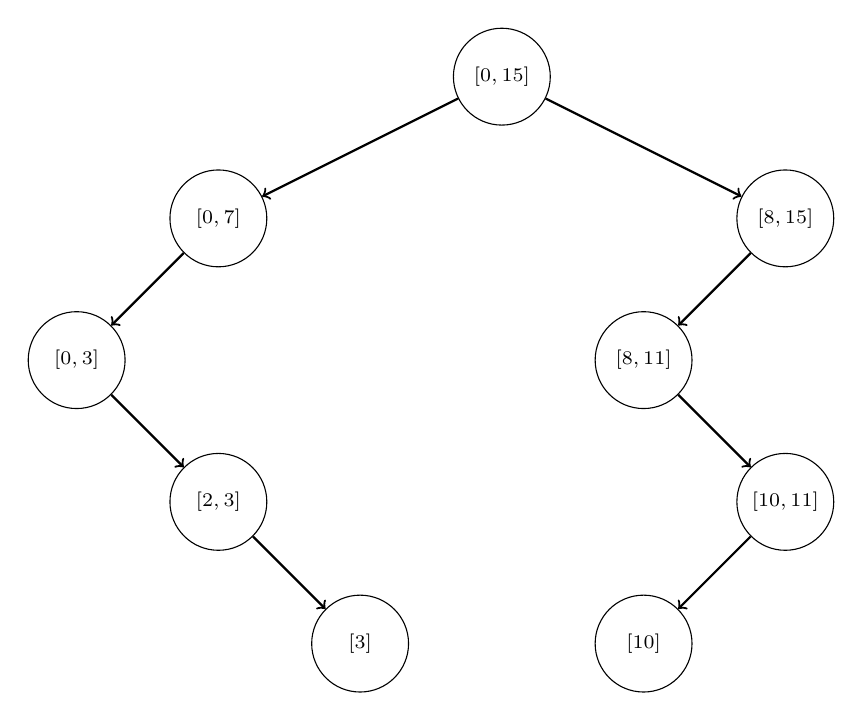
\begin{tikzpicture}[scale=0.9]
\scriptsize
\node[draw, circle,minimum size=35pt] (1) at (0,0) {$[0,15]$};
\node[draw, circle,minimum size=35pt] (2) at (-4,-2) {$[0,7]$};
\node[draw, circle,minimum size=35pt] (3) at (-6,-4) {$[0,3]$};
\node[draw, circle,minimum size=35pt] (4) at (-4,-6) {$[2,3]$};
\node[draw, circle,minimum size=35pt] (5) at (-2,-8) {$[3]$};
\node[draw, circle,minimum size=35pt] (6) at (4,-2) {$[8,15]$};
\node[draw, circle,minimum size=35pt] (7) at (2,-4) {$[8,11]$};
\node[draw, circle,minimum size=35pt] (8) at (4,-6) {$[10,11]$};
\node[draw, circle,minimum size=35pt] (9) at (2,-8) {$[10]$};

\path[draw,thick,->] (1) -- (2);
\path[draw,thick,->] (2) -- (3);
\path[draw,thick,->] (3) -- (4);
\path[draw,thick,->] (4) -- (5);

\path[draw,thick,->] (1) -- (6);
\path[draw,thick,->] (6) -- (7);
\path[draw,thick,->] (7) -- (8);
\path[draw,thick,->] (8) -- (9);
\end{tikzpicture}
\end{center}

Reitti puun juuresta lehteen sisältää
$O(\log N)$ solmua,
joten jokainen muutos puuhun lisää
enintään $O(\log N)$ uutta solmua puuhun.
Niinpä $n$ muutoksen jälkeen puussa
on enintään $O(n \log N)$ solmua.

Huomaa, että jos kaikki tarvittavat indeksit
ovat tiedossa
algoritmin alussa, dynaamisen segmenttipuun
sijasta voi käyttää tavallista segmenttipuuta
ja indeksien pakkausta (luku 9.4).
Tämä ei ole kuitenkaan mahdollista,
jos indeksit syntyvät vasta algoritmin aikana.

\subsection{Muutoshistoria}

Dynaaminen segmenttipuu mahdollistaa myös
puun muutoshistorian säilyttämiseen.
Tämä tarkoittaa, että muistissa on jokainen
segmenttipuun vaihe, joka on esiintynyt
algoritmin suorituksen aikana.

Muutoshistorian hyötynä on,
että kaikkia vanhoja puita voi käsitellä
segmenttipuun tapaan,
koska niiden rakenne on edelleen olemassa.
Vanhoista puista voi myös johtaa uusia
puita, joita voi muokata edelleen.

Tarkastellaan esimerkiksi seuraavaa muutossarjaa,
jossa punaiset solmut muuttuvat päivityksessä
ja muut solmut säilyvät ennallaan:
\\
\begin{center}
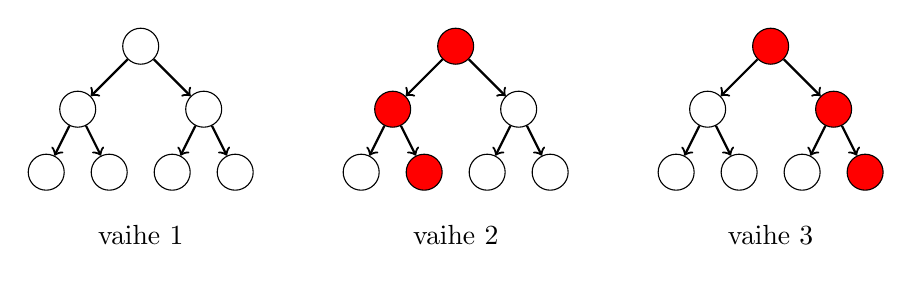
\begin{tikzpicture}[scale=0.8]
\node[draw, circle,minimum size=13pt] (1a) at (3,0) {};
\node[draw, circle,minimum size=13pt] (2a) at (2,-1) {};
\node[draw, circle,minimum size=13pt] (3a) at (4,-1) {};
\node[draw, circle,minimum size=13pt] (4a) at (1.5,-2) {};
\node[draw, circle,minimum size=13pt] (5a) at (2.5,-2) {};
\node[draw, circle,minimum size=13pt] (6a) at (3.5,-2) {};
\node[draw, circle,minimum size=13pt] (7a) at (4.5,-2) {};
\path[draw,thick,->] (1a) -- (2a);
\path[draw,thick,->] (1a) -- (3a);
\path[draw,thick,->] (2a) -- (4a);
\path[draw,thick,->] (2a) -- (5a);
\path[draw,thick,->] (3a) -- (6a);
\path[draw,thick,->] (3a) -- (7a);

\node[draw, circle,minimum size=13pt,fill=red] (1b) at (3+5,0) {};
\node[draw, circle,minimum size=13pt,fill=red] (2b) at (2+5,-1) {};
\node[draw, circle,minimum size=13pt] (3b) at (4+5,-1) {};
\node[draw, circle,minimum size=13pt] (4b) at (1.5+5,-2) {};
\node[draw, circle,minimum size=13pt,fill=red] (5b) at (2.5+5,-2) {};
\node[draw, circle,minimum size=13pt] (6b) at (3.5+5,-2) {};
\node[draw, circle,minimum size=13pt] (7b) at (4.5+5,-2) {};
\path[draw,thick,->] (1b) -- (2b);
\path[draw,thick,->] (1b) -- (3b);
\path[draw,thick,->] (2b) -- (4b);
\path[draw,thick,->] (2b) -- (5b);
\path[draw,thick,->] (3b) -- (6b);
\path[draw,thick,->] (3b) -- (7b);

\node[draw, circle,minimum size=13pt,fill=red] (1c) at (3+10,0) {};
\node[draw, circle,minimum size=13pt] (2c) at (2+10,-1) {};
\node[draw, circle,minimum size=13pt,fill=red] (3c) at (4+10,-1) {};
\node[draw, circle,minimum size=13pt] (4c) at (1.5+10,-2) {};
\node[draw, circle,minimum size=13pt] (5c) at (2.5+10,-2) {};
\node[draw, circle,minimum size=13pt] (6c) at (3.5+10,-2) {};
\node[draw, circle,minimum size=13pt,fill=red] (7c) at (4.5+10,-2) {};
\path[draw,thick,->] (1c) -- (2c);
\path[draw,thick,->] (1c) -- (3c);
\path[draw,thick,->] (2c) -- (4c);
\path[draw,thick,->] (2c) -- (5c);
\path[draw,thick,->] (3c) -- (6c);
\path[draw,thick,->] (3c) -- (7c);

\node at (3,-3) {vaihe 1};
\node at (3+5,-3) {vaihe 2};
\node at (3+10,-3) {vaihe 3};
\end{tikzpicture}
\end{center}
Jokaisen muutoksen jälkeen suurin osa puun
solmuista säilyy ennallaan.
Muistia säästävä tapa tallentaa muutoshistoria
onkin käyttää mahdollisimman paljon hyväksi
puun vanhoja osia muutoksissa.

Tässä tapauksessa muutoshistorian voisi
tallentaa seuraavasti:
\\
\begin{center}
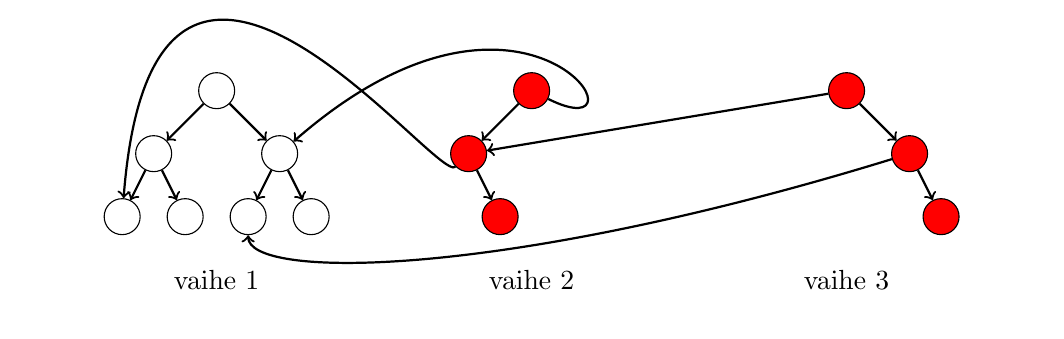
\begin{tikzpicture}[scale=0.8]
\path[use as bounding box] (0, 1) rectangle (16, -3.5);

\node[draw, circle,minimum size=13pt] (1a) at (3,0) {};
\node[draw, circle,minimum size=13pt] (2a) at (2,-1) {};
\node[draw, circle,minimum size=13pt] (3a) at (4,-1) {};
\node[draw, circle,minimum size=13pt] (4a) at (1.5,-2) {};
\node[draw, circle,minimum size=13pt] (5a) at (2.5,-2) {};
\node[draw, circle,minimum size=13pt] (6a) at (3.5,-2) {};
\node[draw, circle,minimum size=13pt] (7a) at (4.5,-2) {};
\path[draw,thick,->] (1a) -- (2a);
\path[draw,thick,->] (1a) -- (3a);
\path[draw,thick,->] (2a) -- (4a);
\path[draw,thick,->] (2a) -- (5a);
\path[draw,thick,->] (3a) -- (6a);
\path[draw,thick,->] (3a) -- (7a);

\node[draw, circle,minimum size=13pt,fill=red] (1b) at (3+5,0) {};
\node[draw, circle,minimum size=13pt,fill=red] (2b) at (2+5,-1) {};
\node[draw, circle,minimum size=13pt,fill=red] (5b) at (2.5+5,-2) {};
\path[draw,thick,->] (1b) -- (2b);

\draw[thick,->] (1b) .. controls (3+5+2,0-1) and (3+5,2.5) .. (3a);

\draw[thick,->] (2b) .. controls (2+5-0.5,-1-0.5) and (2,4.5) .. (4a);


\path[draw,thick,->] (2b) -- (5b);

\node[draw, circle,minimum size=13pt,fill=red] (1c) at (3+10,0) {};
\node[draw, circle,minimum size=13pt,fill=red] (3c) at (4+10,-1) {};
\node[draw, circle,minimum size=13pt,fill=red] (7c) at (4.5+10,-2) {};
\path[draw,thick,->] (1c) -- (2b);
\path[draw,thick,->] (1c) -- (3c);

\draw[thick,->] (3c) .. controls (2.5+5,-3) and (3.5,-3) .. (6a);

\path[draw,thick,->] (3c) -- (7c);

\node at (3,-3) {vaihe 1};
\node at (3+5,-3) {vaihe 2};
\node at (3+10,-3) {vaihe 3};
\end{tikzpicture}
\end{center}

Nyt muistissa on jokaisesta puun vaiheesta
puun juuri, jonka avulla pystyy selvittämään
koko puun rakenteen kyseisellä hetkellä.
Jokainen muutos tuo vain $O(\log N)$ uutta solmua puuhun,
kun puun indeksialue on $[0,N-1]$,
joten koko muutoshistorian pitäminen muistissa on mahdollista.

\section{Tietorakenne solmussa}

Segmenttipuun solmussa voi olla
yksittäisen arvon
sijasta myös jokin tietorakenne,
joka pitää yllä tietoa solmua vastaavasta välistä.
Tällöin segmenttipuun operaatiot vievät aikaa
$O(f(n) \log n)$, missä $f(n)$ on
yksittäisen solmun tietorakenteen
käsittelyyn kuluva aika.

\subsection{Lukumäärät}

\textit{Tehtävä:}
Toteuta segmenttipuu, jonka avulla voi laskea,
montako kertaa luku $x$ esiintyy välillä $[a,b]$.

Ideana on, että jokainen segmenttipuun solmu
sisältää tietorakenteen, josta voi kysyä,
montako kertaa luku $x$ esiintyy kyseisellä välillä.
Vastaus kyselyyn syntyy laskemalla yhteen
esiintymismäärät väleiltä, joista $[a,b]$ muodostuu.

Sopiva tietorakenne tehtävään on
\texttt{map}-rakenne,
jonka avulla voi pitää kirjaa välillä esiintyvien
lukujen määrästä.
Yhden solmun käsittely
vie aikaa $O(\log n)$, joten kunkin
kyselyn aikavaativuus on $O(\log^2 n)$.

Solmuissa olevat tietorakenteet kasvattavat
segmenttipuun muistinkäyttöä.
Tässä tapauksessa
segmenttipuu vie tilaa $O(n \log n)$,
koska siinä on $O(\log n)$ tasoa, joista
jokaisella binääripuut sisältävät $O(n)$ lukua.

Esimerkiksi taulukosta
\begin{center}
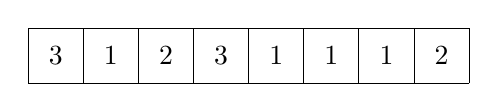
\begin{tikzpicture}[scale=0.7]
\draw (0,0) grid (8,1);

\node[anchor=center] at (0.5, 0.5) {3};
\node[anchor=center] at (1.5, 0.5) {1};
\node[anchor=center] at (2.5, 0.5) {2};
\node[anchor=center] at (3.5, 0.5) {3};
\node[anchor=center] at (4.5, 0.5) {1};
\node[anchor=center] at (5.5, 0.5) {1};
\node[anchor=center] at (6.5, 0.5) {1};
\node[anchor=center] at (7.5, 0.5) {2};
\end{tikzpicture}
\end{center}
syntyy seuraava segmenttipuu:
\begin{center}
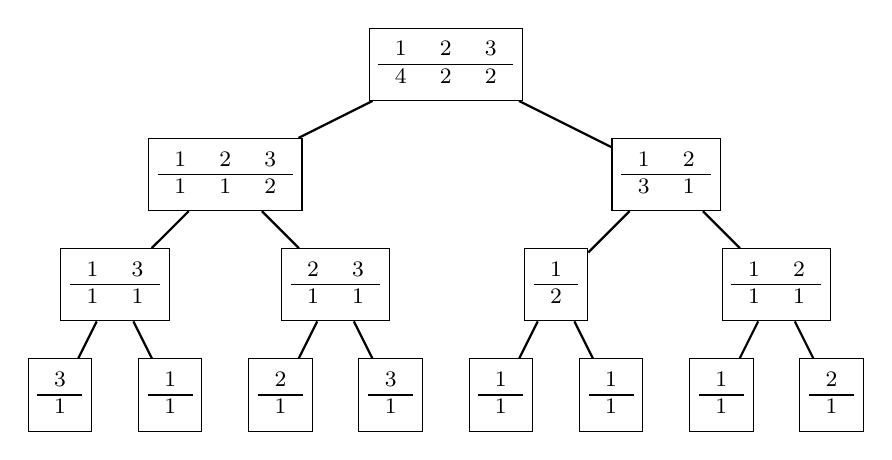
\begin{tikzpicture}[scale=0.7]

\node[draw, rectangle] (a) at (1,2.5)
{
\footnotesize
\begin{tabular}{r}
3 \\
\hline
1 \\
\end{tabular}};
\node[draw, rectangle] (b) at (3,2.5)
{
\footnotesize
\begin{tabular}{r}
1 \\
\hline
1 \\
\end{tabular}};
\node[draw, rectangle] (c) at (5,2.5)
{
\footnotesize
\begin{tabular}{r}
2 \\
\hline
1 \\
\end{tabular}};
\node[draw, rectangle] (d) at (7,2.5)
{
\footnotesize
\begin{tabular}{r}
3 \\
\hline
1 \\
\end{tabular}};
\node[draw, rectangle] (e) at (9,2.5)
{
\footnotesize
\begin{tabular}{r}
1 \\
\hline
1 \\
\end{tabular}};
\node[draw, rectangle] (f) at (11,2.5)
{
\footnotesize
\begin{tabular}{r}
1 \\
\hline
1 \\
\end{tabular}};
\node[draw, rectangle] (g) at (13,2.5)
{
\footnotesize
\begin{tabular}{r}
1 \\
\hline
1 \\
\end{tabular}};
\node[draw, rectangle] (h) at (15,2.5)
{
\footnotesize
\begin{tabular}{r}
2 \\
\hline
1 \\
\end{tabular}};

\node[draw, rectangle] (i) at (2,4.5)
{
\footnotesize
\begin{tabular}{rr}
1 & 3 \\
\hline
1 & 1 \\
\end{tabular}};
\path[draw,thick,-] (i) -- (a);
\path[draw,thick,-] (i) -- (b);
\node[draw, rectangle] (j) at (6,4.5)
{
\footnotesize
\begin{tabular}{rr}
2 & 3 \\
\hline
1 & 1 \\
\end{tabular}};
\path[draw,thick,-] (j) -- (c);
\path[draw,thick,-] (j) -- (d);
\node[draw, rectangle] (k) at (10,4.5)
{
\footnotesize
\begin{tabular}{r}
1 \\
\hline
2 \\
\end{tabular}};
\path[draw,thick,-] (k) -- (e);
\path[draw,thick,-] (k) -- (f);
\node[draw, rectangle] (l) at (14,4.5)
{
\footnotesize
\begin{tabular}{rr}
1 & 2 \\
\hline
1 & 1 \\
\end{tabular}};
\path[draw,thick,-] (l) -- (g);
\path[draw,thick,-] (l) -- (h);

\node[draw, rectangle] (m) at (4,6.5)
{
\footnotesize
\begin{tabular}{rrr}
1 & 2 & 3 \\
\hline
1 & 1 & 2 \\
\end{tabular}};
\path[draw,thick,-] (m) -- (i);
\path[draw,thick,-] (m) -- (j);
\node[draw, rectangle] (n) at (12,6.5)
{
\footnotesize
\begin{tabular}{rr}
1 & 2 \\
\hline
3 & 1 \\
\end{tabular}};
\path[draw,thick,-] (n) -- (k);
\path[draw,thick,-] (n) -- (l);

\node[draw, rectangle] (o) at (8,8.5)
{
\footnotesize
\begin{tabular}{rrr}
1 & 2 & 3 \\
\hline
4 & 2 & 2 \\
\end{tabular}};
\path[draw,thick,-] (o) -- (m);
\path[draw,thick,-] (o) -- (n);
\end{tikzpicture}
\end{center}

\subsection{Kaksiulotteisuus}

\textit{Tehtävä:}
Toteuta segmenttipuu, jolla pystyy laskemaan
$n \times n$ -kokoisen
kaksi\-ulotteisen taulukon alitaulukon
summan sekä muuttamaan taulukkoa.

Tavallinen tapa toteuttaa kaksiulotteinen
segmenttipuu on luoda segmenttipuu,
jonka jokaisessa solmussa on segmenttipuu.
Suuri segmenttipuu vastaa taulukon rivejä,
ja pienet segmenttipuut vastaavat sarakkeita.

\newpage
Esimerkiksi taulukon
\\
\begin{center}
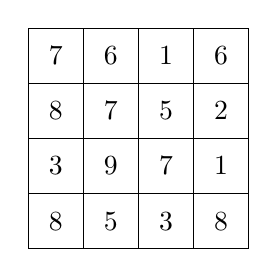
\begin{tikzpicture}[scale=0.7]
\draw (0,0) grid (4,4);

\node[anchor=center] at (0.5, 0.5) {8};
\node[anchor=center] at (1.5, 0.5) {5};
\node[anchor=center] at (2.5, 0.5) {3};
\node[anchor=center] at (3.5, 0.5) {8};

\node[anchor=center] at (0.5, 1.5) {3};
\node[anchor=center] at (1.5, 1.5) {9};
\node[anchor=center] at (2.5, 1.5) {7};
\node[anchor=center] at (3.5, 1.5) {1};

\node[anchor=center] at (0.5, 2.5) {8};
\node[anchor=center] at (1.5, 2.5) {7};
\node[anchor=center] at (2.5, 2.5) {5};
\node[anchor=center] at (3.5, 2.5) {2};

\node[anchor=center] at (0.5, 3.5) {7};
\node[anchor=center] at (1.5, 3.5) {6};
\node[anchor=center] at (2.5, 3.5) {1};
\node[anchor=center] at (3.5, 3.5) {6};
\end{tikzpicture}
\end{center}

alueiden summia voi laskea seuraavasta segmenttipuusta:
\\
\begin{center}
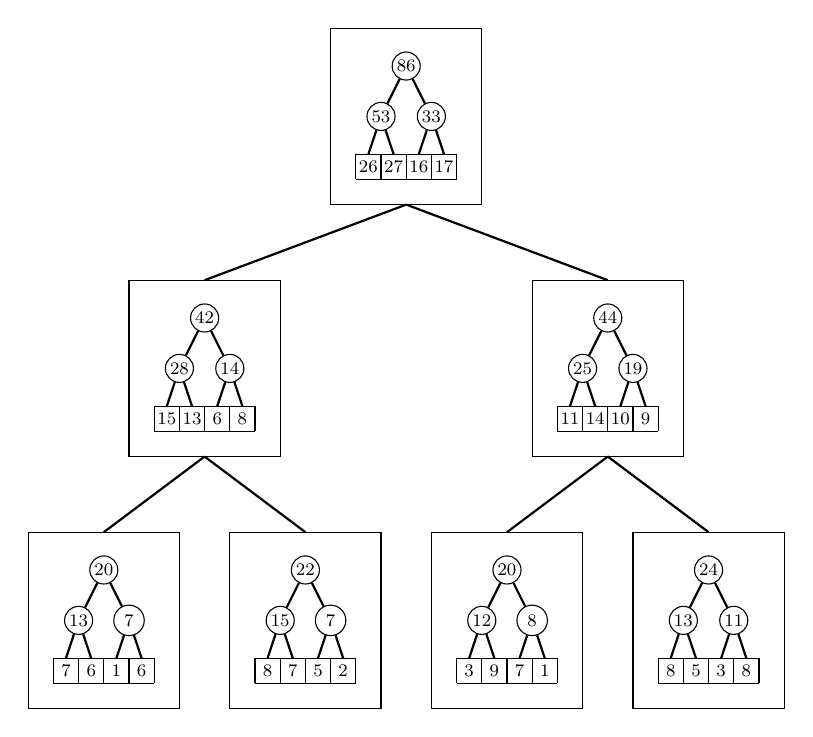
\begin{tikzpicture}[scale=0.32]
\footnotesize
\begin{scope}[shift={(-12,0)}]
\draw (-1,-1) rectangle (5,6);
\draw (0,0) grid (4,1);
\node[anchor=center,scale=0.8] at (0.5, 0.5) {7};
\node[anchor=center,scale=0.8] at (1.5, 0.5) {6};
\node[anchor=center,scale=0.8] at (2.5, 0.5) {1};
\node[anchor=center,scale=0.8] at (3.5, 0.5) {6};

\node[draw, circle,scale=0.8,inner sep=1pt] (a) at (1,2.5) {13};
\path[draw,thick,-] (a) -- (0.5,1);
\path[draw,thick,-] (a) -- (1.5,1);
\node[draw, circle,scale=0.8,inner sep=2.5pt] (b) at (3,2.5) {7};
\path[draw,thick,-] (b) -- (2.5,1);
\path[draw,thick,-] (b) -- (3.5,1);

\node[draw, circle,scale=0.8,inner sep=1pt] (i) at (2,4.5) {20};
\path[draw,thick,-] (i) -- (a);
\path[draw,thick,-] (i) -- (b);
\end{scope}
\begin{scope}[shift={(-4,0)}]
\draw (-1,-1) rectangle (5,6);
\draw (0,0) grid (4,1);
\node[anchor=center,scale=0.8] at (0.5, 0.5) {8};
\node[anchor=center,scale=0.8] at (1.5, 0.5) {7};
\node[anchor=center,scale=0.8] at (2.5, 0.5) {5};
\node[anchor=center,scale=0.8] at (3.5, 0.5) {2};

\node[draw, circle,scale=0.8,inner sep=1pt] (a) at (1,2.5) {15};
\path[draw,thick,-] (a) -- (0.5,1);
\path[draw,thick,-] (a) -- (1.5,1);
\node[draw, circle,scale=0.8,inner sep=2.5pt] (b) at (3,2.5) {7};
\path[draw,thick,-] (b) -- (2.5,1);
\path[draw,thick,-] (b) -- (3.5,1);

\node[draw, circle,scale=0.8,inner sep=1pt] (i) at (2,4.5) {22};
\path[draw,thick,-] (i) -- (a);
\path[draw,thick,-] (i) -- (b);
\end{scope}
\begin{scope}[shift={(4,0)}]
\draw (-1,-1) rectangle (5,6);
\draw (0,0) grid (4,1);
\node[anchor=center,scale=0.8] at (0.5, 0.5) {3};
\node[anchor=center,scale=0.8] at (1.5, 0.5) {9};
\node[anchor=center,scale=0.8] at (2.5, 0.5) {7};
\node[anchor=center,scale=0.8] at (3.5, 0.5) {1};

\node[draw, circle,scale=0.8,inner sep=1pt] (a) at (1,2.5) {12};
\path[draw,thick,-] (a) -- (0.5,1);
\path[draw,thick,-] (a) -- (1.5,1);
\node[draw, circle,scale=0.8,inner sep=2.5pt] (b) at (3,2.5) {8};
\path[draw,thick,-] (b) -- (2.5,1);
\path[draw,thick,-] (b) -- (3.5,1);

\node[draw, circle,scale=0.8,inner sep=1pt] (i) at (2,4.5) {20};
\path[draw,thick,-] (i) -- (a);
\path[draw,thick,-] (i) -- (b);
\end{scope}
\begin{scope}[shift={(12,0)}]
\draw (-1,-1) rectangle (5,6);
\draw (0,0) grid (4,1);
\node[anchor=center,scale=0.8] at (0.5, 0.5) {8};
\node[anchor=center,scale=0.8] at (1.5, 0.5) {5};
\node[anchor=center,scale=0.8] at (2.5, 0.5) {3};
\node[anchor=center,scale=0.8] at (3.5, 0.5) {8};

\node[draw, circle,scale=0.8,inner sep=1pt] (a) at (1,2.5) {13};
\path[draw,thick,-] (a) -- (0.5,1);
\path[draw,thick,-] (a) -- (1.5,1);
\node[draw, circle,scale=0.8,inner sep=1pt] (b) at (3,2.5) {11};
\path[draw,thick,-] (b) -- (2.5,1);
\path[draw,thick,-] (b) -- (3.5,1);

\node[draw, circle,scale=0.8,inner sep=1pt] (i) at (2,4.5) {24};
\path[draw,thick,-] (i) -- (a);
\path[draw,thick,-] (i) -- (b);
\end{scope}
\begin{scope}[shift={(-8,10)}]
\draw (-1,-1) rectangle (5,6);
\draw (0,0) grid (4,1);
\node[anchor=center,scale=0.8] at (0.5, 0.5) {15};
\node[anchor=center,scale=0.8] at (1.5, 0.5) {13};
\node[anchor=center,scale=0.8] at (2.5, 0.5) {6};
\node[anchor=center,scale=0.8] at (3.5, 0.5) {8};

\node[draw, circle,scale=0.8,inner sep=1pt] (a) at (1,2.5) {28};
\path[draw,thick,-] (a) -- (0.5,1);
\path[draw,thick,-] (a) -- (1.5,1);
\node[draw, circle,scale=0.8,inner sep=1pt] (b) at (3,2.5) {14};
\path[draw,thick,-] (b) -- (2.5,1);
\path[draw,thick,-] (b) -- (3.5,1);

\node[draw, circle,scale=0.8,inner sep=1pt] (i) at (2,4.5) {42};
\path[draw,thick,-] (i) -- (a);
\path[draw,thick,-] (i) -- (b);
\end{scope}
\begin{scope}[shift={(8,10)}]
\draw (-1,-1) rectangle (5,6);
\draw (0,0) grid (4,1);
\node[anchor=center,scale=0.8] at (0.5, 0.5) {11};
\node[anchor=center,scale=0.8] at (1.5, 0.5) {14};
\node[anchor=center,scale=0.8] at (2.5, 0.5) {10};
\node[anchor=center,scale=0.8] at (3.5, 0.5) {9};

\node[draw, circle,scale=0.8,inner sep=1pt] (a) at (1,2.5) {25};
\path[draw,thick,-] (a) -- (0.5,1);
\path[draw,thick,-] (a) -- (1.5,1);
\node[draw, circle,scale=0.8,inner sep=1pt] (b) at (3,2.5) {19};
\path[draw,thick,-] (b) -- (2.5,1);
\path[draw,thick,-] (b) -- (3.5,1);

\node[draw, circle,scale=0.8,inner sep=1pt] (i) at (2,4.5) {44};
\path[draw,thick,-] (i) -- (a);
\path[draw,thick,-] (i) -- (b);
\end{scope}
\begin{scope}[shift={(0,20)}]
\draw (-1,-1) rectangle (5,6);
\draw (0,0) grid (4,1);
\node[anchor=center,scale=0.8] at (0.5, 0.5) {26};
\node[anchor=center,scale=0.8] at (1.5, 0.5) {27};
\node[anchor=center,scale=0.8] at (2.5, 0.5) {16};
\node[anchor=center,scale=0.8] at (3.5, 0.5) {17};

\node[draw, circle,scale=0.8,inner sep=1pt] (a) at (1,2.5) {53};
\path[draw,thick,-] (a) -- (0.5,1);
\path[draw,thick,-] (a) -- (1.5,1);
\node[draw, circle,scale=0.8,inner sep=1pt] (b) at (3,2.5) {33};
\path[draw,thick,-] (b) -- (2.5,1);
\path[draw,thick,-] (b) -- (3.5,1);

\node[draw, circle,scale=0.8,inner sep=1pt] (i) at (2,4.5) {86};
\path[draw,thick,-] (i) -- (a);
\path[draw,thick,-] (i) -- (b);
\end{scope}
\path[draw,thick,-] (2,19) -- (-6,16);
\path[draw,thick,-] (2,19) -- (10,16);
\path[draw,thick,-] (-6,9) -- (-10,6);
\path[draw,thick,-] (-6,9) -- (-2,6);
\path[draw,thick,-] (10,9) -- (6,6);
\path[draw,thick,-] (10,9) -- (14,6);
\end{tikzpicture}
\end{center}

Segmenttipuun operaatiot vievät aikaa
$O(\log^2 n)$,
koska suuressa puussa ja kussakin
pienessä puussa on $O(\log n)$ tasoa.
Segmenttipuu vie muistia $O(n^2)$,
koska jokainen pieni puu
vie muistia $O(n)$.

Vastaavalla tavalla voi luoda myös segmenttipuita,
joissa on vielä enemmän ulottuvuuksia,
mutta tälle on harvoin tarvetta.

